\documentclass[tikz,border=5pt]{standalone}
\usepackage{amsmath}
\usetikzlibrary{positioning, arrows.meta, calc}

\begin{document}

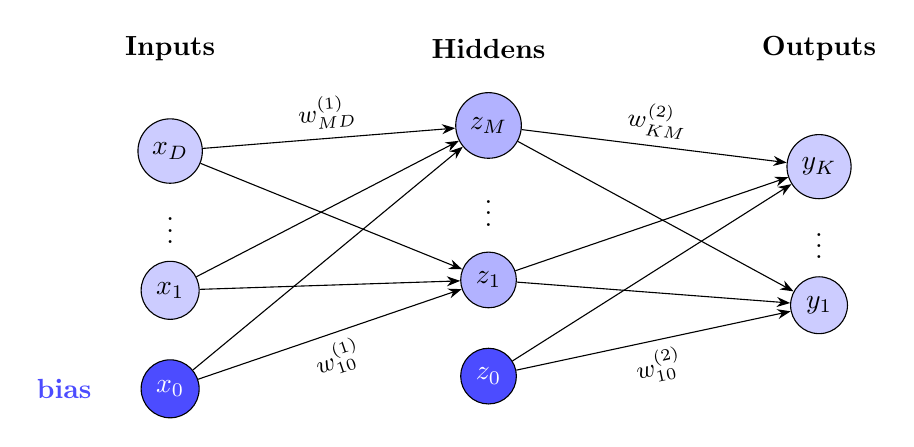
\begin{tikzpicture}[
    node distance=1.2cm and 2.5cm,
    % every node/.style={draw, circle, minimum size=1.2cm, inner sep=0pt},
    input/.style={draw, circle, fill=blue!20},
    hidden/.style={draw, circle, fill=blue!30},
    output/.style={draw, circle, fill=blue!20},
    bias/.style={draw, circle, fill=blue!70, text=white},
    weight/.style={font=\small, midway, below, sloped},
    >=Stealth
]

% --- 输入层 ---
\node[] (inputs) {\textbf{Inputs}};
\node[input, below=0.6cm of inputs] (xD) {$x_D$};
\node[below=0.1cm of xD] (dots1) {$\vdots$};
\node[input, below=0.1cm of dots1] (x1) {$x_1$};
\node[bias, below=0.5cm of x1] (x0) {$x_0$};
\node[left=0.5cm of x0, text=blue!70] (bs) {\textbf{bias}};

% --- 隐藏层 ---
\node[right=of inputs] (hiddens) {\textbf{Hiddens}};
\node[hidden, below=0.3cm of hiddens] (zM) {$z_M$};
\node[below=0.2cm of zM] (dots2) {$\vdots$};
\node[hidden, below=0.2cm of dots2] (z1) {$z_1$};
\node[bias, below=0.5cm of z1] (z0) {$z_0$}; % 偏置

% --- 输出层 ---
\node[right=of hiddens] (outputs) {\textbf{Outputs}};
\node[output, below=0.8cm of outputs] (yK) {$y_K$};
\node[below=0.1cm of yK] (dots3) {$\vdots$};
\node[output, below=0.1cm of dots3] (y1) {$y_1$};

% --- 连接线与权重标注 ---
% 输入 → 隐藏层（第一层权重）
\draw[->] (x0) -- (z1) node[weight]{$w_{10}^{(1)}$};
\draw[->] (x0) -- (zM) node[weight]{}; 
\draw[->] (x1) -- (z1) node[weight]{}; 
\draw[->] (x1) -- (zM) node[weight]{}; 
\draw[->] (xD) -- (z1) node[weight]{}; 
\draw[->] (xD) -- (zM) node[weight, above]{$w_{MD}^{(1)}$}; 

% 隐藏层 → 输出层（第二层权重）
\draw[->] (z1) -- (y1) node[weight]{};
\draw[->] (z1) -- (yK) node[weight]{}; 
\draw[->] (zM) -- (y1) node[weight]{}; 
\draw[->] (zM) -- (yK) node[weight, above]{$w_{KM}^{(2)}$}; 
\draw[->] (z0) -- (y1) node[weight]{$w_{10}^{(2)}$};
\draw[->] (z0) -- (yK) node[weight]{};

% 调整部分权重位置避免重叠（可选微调）
% \path (x0) -- (zM) node[weight, pos=0.4, xshift=-0.7cm, yshift=0.1cm] {$w_{M0}^{(1)}$};

\end{tikzpicture}

\end{document}